\documentclass[english]{proposalnsf}
\usepackage{graphicx}
\usepackage{url}
\usepackage[square,numbers]{natbib}
\usepackage[nottoc,numbib]{tocbibind}

\title{An Ethnographic User Experience Evaluation of RadGrad}
\author{Quinne Uchida \\Collaborative Software Development Laboratory \\ Information and Computer Sciences \\ University of Hawaii}

\begin{document}
\maketitle
\tableofcontents
\newpage

\section{Introduction}
\label{introduction}

The introduction section typically begins with a description of a {\em Big Problem}. The demand for Computer Science jobs is growing rapidly and so is the demand for Computer Science degrees. However, employers are looking for individuals who have been educated in Computer Science, along with experience doing internships, extracurricular activities and other projects. The traditional perception of qualifications for obtaining a job were that one must have a high GPA. RadGrad is designed to address this problem. 

The next part of the introduction section presents the {\em Small Problem}--- Low system adoption of RadGrad. We define low system adoption as 0-1 sessions per semester. We define a moderate level of adoption as 2-3 sessions per semester.  We define the a high level of system adoption as 4 or more sessions per semester. 

According to data collected from RadGrad1 for Spring 2019 (2019-01-01 to 2019-05-31), out of 210 active students, 138 students are classified as having low system adoption. 57 students are classified as having moderate system adoption and 15 classify as having high adoption. In terms of percentage, 65.71{\%} have low adoption, 27.14{\%} have moderate adoption and 7.14{\%} have high adoption, which totals to 99.99{\%}. 

These numbers have been calculated from session data for Spring 2019 (2019-01-01 to 2019-05-31) obtained on 2019-11-20 as reported by the RadGrad system. 

{\em Sessions} are classified as periods of activity deliminated by 1 hour of inactivity. Having an hour of idle time creates a new session. The purpose of defining levels of adoption by number of sessions is because a user's number of login events may not accurately reflect activity of the system.

The final part of the introduction section describes how the rest of this document is organized, which should also lead the reader through your research process.  For example, ``Section \ref{related-work} discusses research related to gender in STEM disciplines including computer science.  Section \ref{research-design} presents the research process I will use in order to gather data related to barriers to completion of a computer science degree program.  Section \ref{results} presents the data I will collect and how I will analyze it.  Section \ref{conclusions} presents my conclusions and proposals for future research.''

\section{Related Work}
\label{related-work}

The Related Work section presents research and/or technology that you are using as a basis for your project.  Related Work sections generally should establish the following:

\begin{itemize}
\item Your research project is novel---no one else has already definitively solved your Small Problem.
\item Your research project is important. You can discuss research that provides more detail about the Big Problem, for example. This might include research on the economic or social costs of the Big Problem.
\item Your research project is important.  Another way to show importance is to discuss research by other people related to your Small Problem, but that doesn't provide all of the insight your project will provide.
\item The technologies you plan to use, or technologies related to what you are going to do. If your project involves technology implementation, then you will want to talk about related technologies in this section.
\end{itemize}


\section{Research Design}
\label{research-design}

We would like to improve the student participation in RadGrad, and by conducting an ethnographic study we may be able to identify and examine barriers of adoption for RadGrad. The main question I will be attempting to answer is: "Why do/don't students use RadGrad?"

In this study, the ethnographer will attempt to interview a total of 5-10 students. For each student, the ethnographer will interview the student for 15 minutes and record audio of the process. After the interview, the ethnographer will then transcribe and analyze the contents of the interview. 

While the ethnographer must allow the interview to change topics if the participant wishes, the ethnographer must still have a plan. Initially, the interviewer will ask the participant about their opinions on RadGrad. From there, the participant has the freedom to talk about any aspect of RadGrad and not a specific category. Theoretically, the first aspect of RadGrad the participant brings up will be the one deemed most important by that participant. 

{\em Pilot Study}
Ethnographic studies are rarely done because of the time commitment required to analyze ethnographic data. I propose conducting a pilot study on 2 students. These students will be subject to the proposed structure of this study and will allow the ethnographer to further refine the proposed process. 

Quite often, you will want to add a picture to your tech report. The trick for including figures into LaTeX is to first convert them to encapsulated postscript (.eps) format. I use the convert program, but for Windows, you might ned pdftoops or ghostscript.  Google for lots of ideas on how to do this. All figures in your tech report must be referenced. So for example, Figure \ref{fig:theory} presents a theory of change for the RadGrad project.

\begin{figure}[t]
  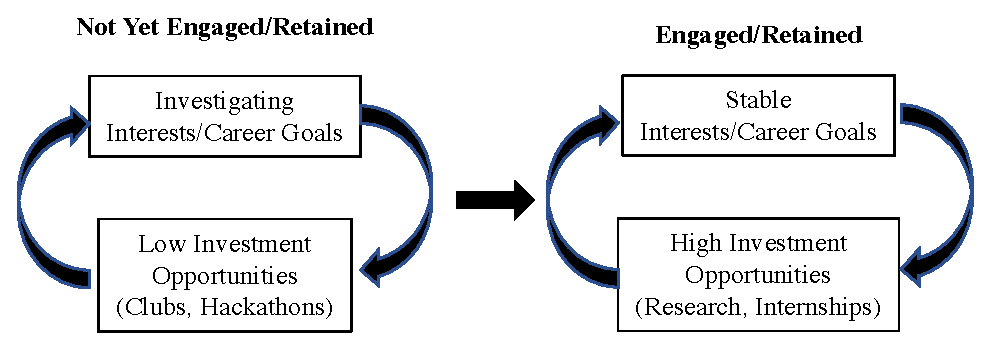
\includegraphics[width=\textwidth]{theory-of-change.eps}
  \caption{Theory of change}
  \label{fig:theory}
\end{figure}

You might also want to include a table.  Figure \ref{fig:hardware-table} shows an example table.

\begin{figure}[ht]
  \begin{tabular}{l|r|p{2in}|p{1in}|p{1in}} \hline
  {\bf Device} & {\bf Cost} & {\bf Measurements} & {\bf Synchronization} & {\bf Communication} \\ \hline
  PMU & \$100,000 & frequency, voltage, current & GPS & Secure LAN  \\
  FDR & \$2,500 & frequency, voltage & GPS & Internet \\
  PQube & \$5,000+ & frequency, voltage, THD, VARs & (none) & (none)  \\
  mPMU & \$5,000+ & frequency, voltage, THD, VARs & GPS & Custom network \\
  AC Scout & \$200+  & frequency, voltage & (none) & (none) \\
  OPQ & \$60 & frequency, voltage, THD & NTP & HTTP/SSE \\
  \hline
  \end{tabular}
  \caption{Comparison of hardware devices for power quality monitoring}
  \label{fig:hardware-table}
\end{figure}


\section{Results}
\label{results}

This section is not needed in a tech report intended as a proposal.  Once you have completed your project, then you can add this section to discuss what results you came up with.

\section{Conclusions}
\label{conclusions}

This is the fun section. Here you get to discuss how the data you collected about the Small Problem has provided some insight into what is needed to resolve the Big Problem.

Even more fun, this section allows you to provide opinions to future generations of researchers in this area. If you were going to continue on, what research question would you pursue next?  If you were going to repeat this project, what would you change about its design, now that you know what you know?


\bibliography{techreport}
\bibliographystyle{plainnat}

\appendix
\section{Formatting tips}

One of the most common mistakes by newcomers to LaTeX is forgetting to escape the percent and dollar sign characters. The percent character (\%) comments out the rest of the current line, while the dollar sign character (\$) puts LaTeX into math mode, which is often not what you want. Put a backslash before them to get these characters to print normally.

\end{document}

